\documentclass[letterpaper]{article} 
\usepackage[left = 0.5in, right = 0.5in, top = 0.9in, bottom = 0.9in]{geometry}
\usepackage{enumitem}
\usepackage{multicol}
\usepackage[spanish]{babel}
\usepackage[utf8]{inputenc}

\usepackage{amsmath,amssymb,amsthm}
\usepackage{tikz-cd}
\usepackage{mathrsfs}
\usepackage[bbgreekl]{mathbbol}
\usepackage{dsfont}
\usepackage{listings}
\usepackage{graphicx}
\graphicspath{{img/}}

\newcommand{\op}{\operatorname}
\newcommand{\Op}{^{\op{op}}}
\newcommand{\scc}{\mathscr C}
\newcommand{\scd}{\mathscr D}
\newcommand{\sce}{\mathscr E}
\newcommand{\sci}{\mathscr I}
\newcommand{\scj}{\mathscr J}
\newcommand{\scx}{\mathscr X}
\newcommand{\var}{\mathrm{Var}}
\newcommand{\Id}{\operatorname{Id}}
\newcommand{\N}{\mathbb N}
\newcommand{\Z}{\mathbb Z}
\newcommand{\Q}{\mathbb{Q}}
\newcommand{\I}{\mathbb{I}}
\newcommand{\R}{\mathbb{R}}
\newcommand{\C}{\mathbb{C}}
\newcommand{\F}{\mathcal{F}}
\newcommand{\G}{\mathcal{G}}
\newcommand{\B}{\mathcal{B}}
\newcommand{\abs}[1]{\left\lvert #1 \right\rvert}
\newcommand{\inv}{^{-1}}
\renewcommand{\to}{\rightarrow}
\newcommand{\ent}{\Longrightarrow}
\newcommand{\E}{\mathbb{E}}
\renewcommand{\P}{\mathbb{P}}
\newcommand{\1}{\mathds{1}}
\renewcommand{\qedsymbol}{$\blacksquare$}

\theoremstyle{definition}
\newtheorem{dfn}{Definición}
\theoremstyle{definition}
\newtheorem{teo}{Teorema}
\theoremstyle{definition}
\newtheorem{cor}{Corolario}
\theoremstyle{definition}
\newtheorem{prop}{Proposición}
\theoremstyle{definition}
\newtheorem{obs}{Observación}


\title{\textbf{Cómputo Científico\\Tarea 2\\Descomposición QR y mínimos cuadrados}}
\author{Iván Irving Rosas Domínguez}
\date{\today}

\DeclareSymbolFontAlphabet{\mathbbm}{bbold}
\DeclareSymbolFontAlphabet{\mathbb}{AMSb}
\DeclareMathSymbol\bbDelta  \mathord{bbold}{"01}

\begin{document}
\maketitle

%\begin{abstract}
%\end{abstract}

\begin{enumerate}
    \item Implementar el algoritmo de Gram-Schmidt modificado 8.1 del Trefethen (p. 58)
    para generar la descomposición $QR$.\\

    \textbf{Solución:} Este algoritmo se implementó con el nombre de 'GMmodificado', el cual hace alusión
    al método para crear la base ortonormal que se calcula en el procedimiento. Este código se puede ver 
    en el script 'GM modificado'. Como recordatorio, observemos que nosotros estamos hallando la descomposición
    $QR$ reducida, es decir
    \[
    A=\hat{Q}\hat{R}.
    \]
    
    \item Implementar el algoritmo que calcula el estimador de mínimos cuadrados
    en una regresión usando la descomposición $QR$.\\

    \textbf{Solución:} Este algoritmo se implementó con el nombre de 'QRsol', y se puede encontrar en 
    el script 'Minimos cuadrados' de esta tarea.\\

    Como nota técnica, el algoritmo realiza la descomposición $A=QR$, de tal forma que para 'solucionar' el
    sistema $Ax=y$, se realiza lo siguiente:
    \[
    Ax=y \quad \ent \quad QRx=y \quad \ent \quad Q^*QRx=Q^*y \quad \ent \quad Rx=Q^*y,
    \]
    por lo que solucionar $Ax=y$ equivale a solucionar $Rx=Q^*y$, pero ya conocemos $R$, por lo que
    solo resta hallar $Q^*y$, lo cual es sencillo pues simplemente transponemos $Q$ de la factorización
    $QR$ y terminamos.

    \item Generar $\textbf{Y}$ compuesto de $y_i=\sen(x_i)+\varepsilon_i$, donde 
    $\varepsilon_i\sim N(0,\sigma^2)$, con $\sigma=0.11$ para $x_i=\frac{4\pi i}{n}$,
    para $i\in \left\{1,...,n\right\}$.
    Hacer un ajuste de mínimos cuadrados a $\textbf{Y}$, con descomposición $QR$,
    ajustando un polinomio de grado $p-1$.
    \begin{itemize}
        \item Considerar los 12 casos: $p=3,4,6,100$ y $n=100,1000,10000$.
        \item Graficar el ajuste en cada caso.
        \item Medir el tiempo de ejecución de su algoritmo, comparar con 
        descomposición $QR$ de scipy y graficar los resultados.
    \end{itemize}
    \textbf{Solución:} Consideramos los 12 casos que se nos pueden presentar. En nuestra presentación elegimos la variable $m$ como la variable
    $n$ mencionada en este ejercicio, para mayor familiaridad con una matriz de $m\times n$, $m$ observaciones, $n$ regresores.\\

    El script relacionado con este ejercicio se denomina 'Ejercicio 3', y en él se encuentran los algoritmos para crear
    una matriz de Vandermonde, realizar la regresión, y el ajuste polinomial con cualesquiera parámetros $m$, y $p$, siempre que
    sean adecuados $m\geq p-1$. Después de realizar el siguiente ajuste, obtenemos las siguientes gráficas para cada uno de los 
    casos:

    \begin{figure}[h]
        \centering
        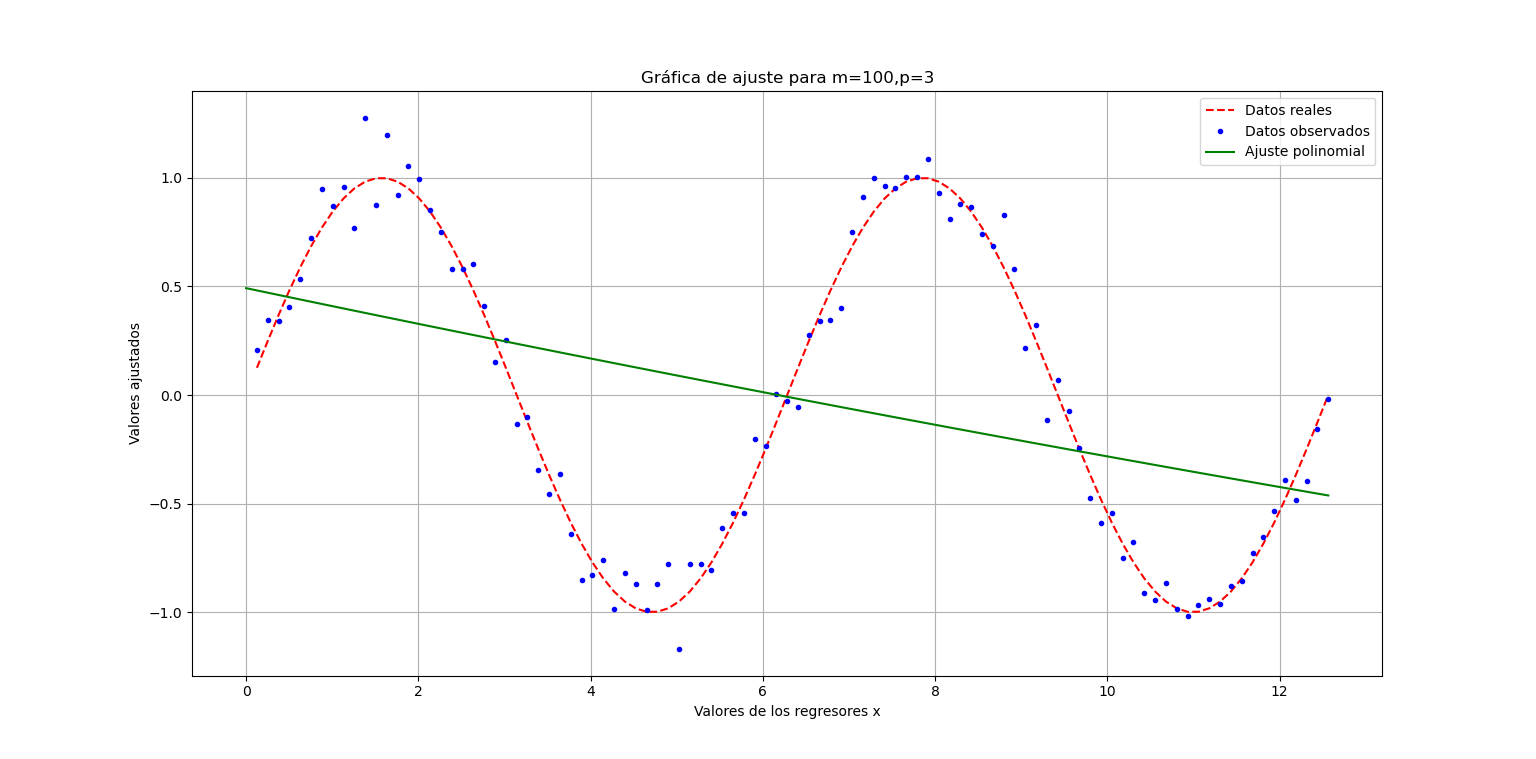
\includegraphics[width=0.7\linewidth]{1.png}
        \caption{}
    \end{figure}
    \begin{figure}[h]
        \centering
        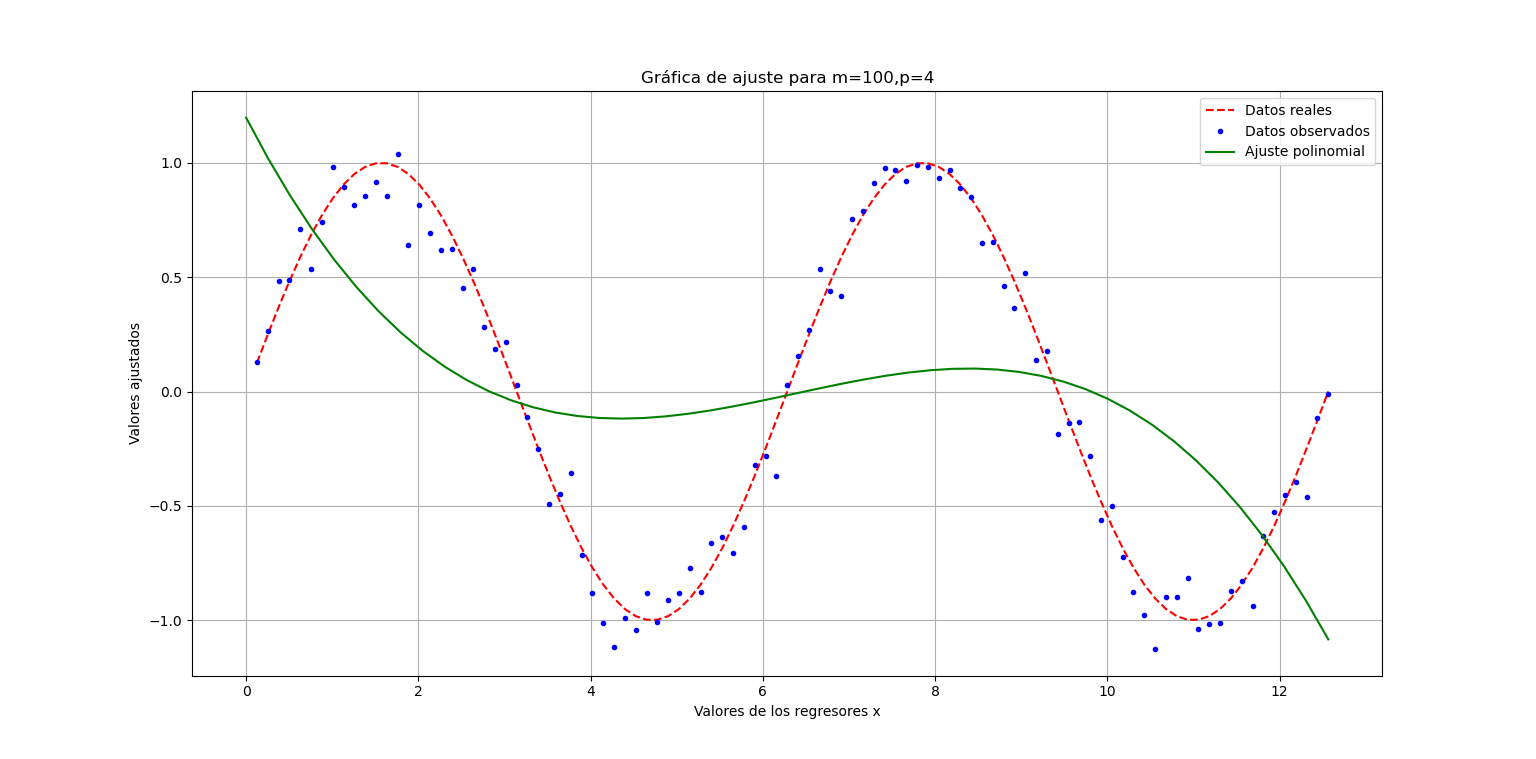
\includegraphics[width=0.7\linewidth]{2.png}
        \caption{}
    \end{figure}  
    \begin{figure}[h]
        \centering
        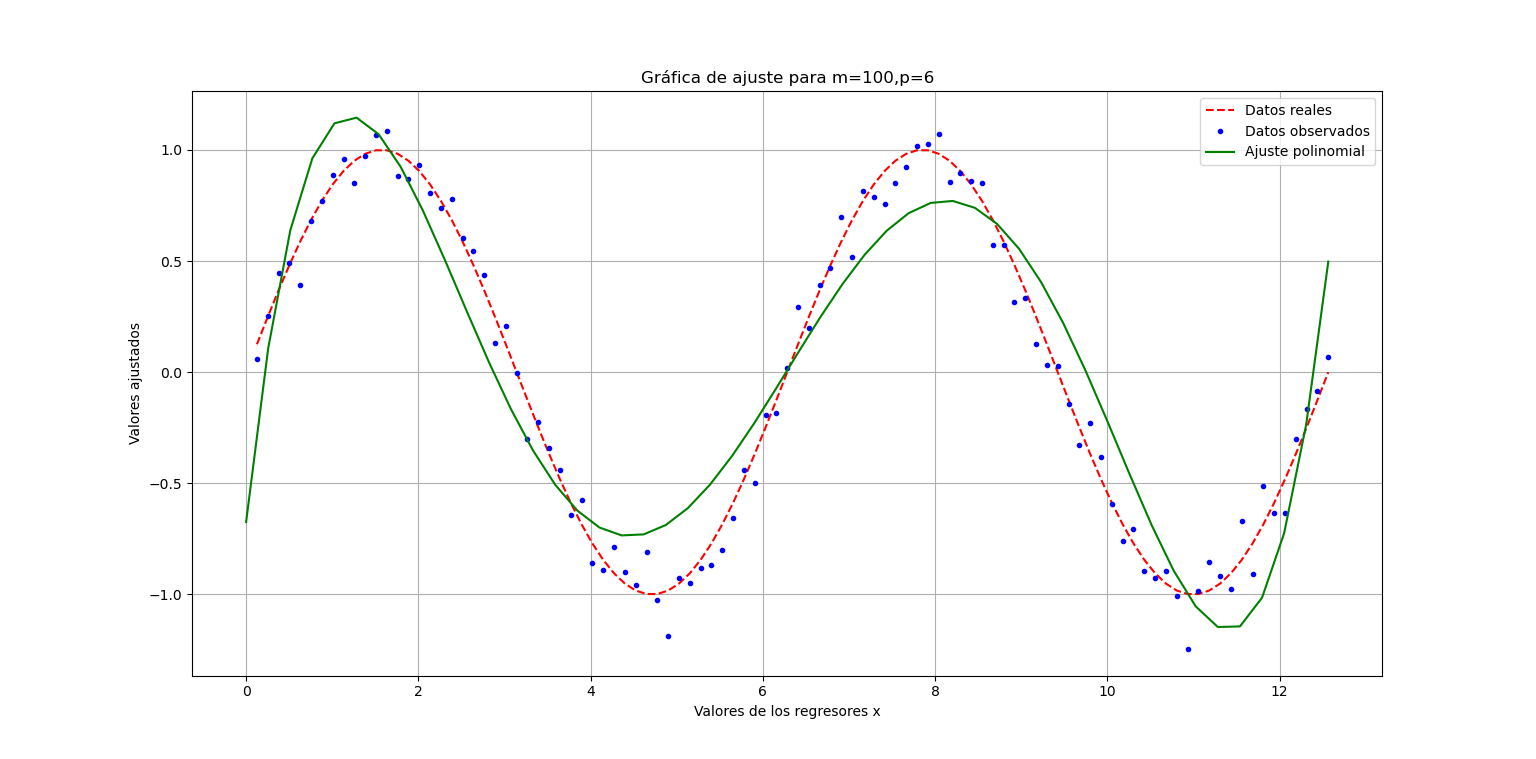
\includegraphics[width=0.7\linewidth]{3.png}
        \caption{}
    \end{figure}  
    \begin{figure}[h]
        \centering
        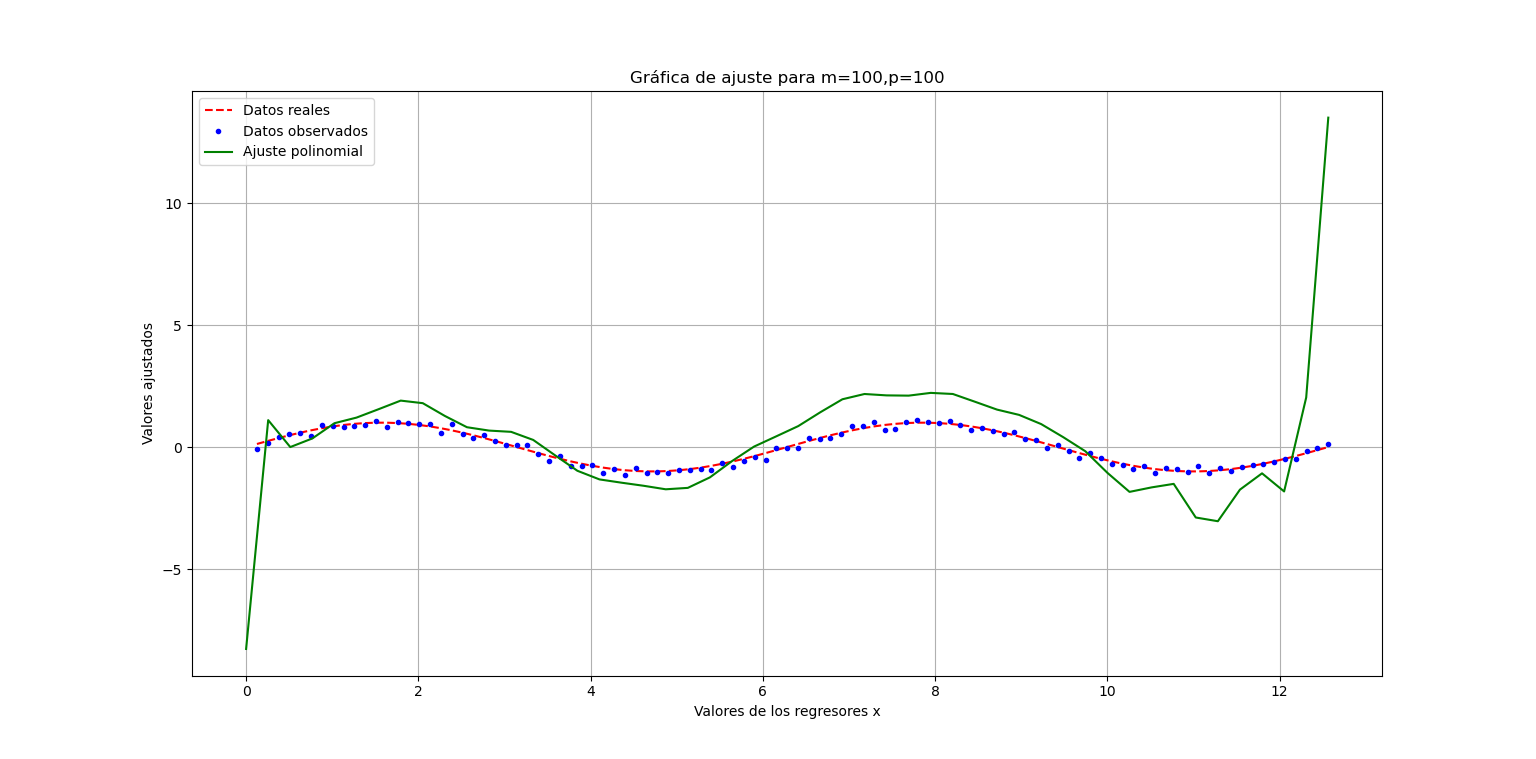
\includegraphics[width=0.7\linewidth]{4.png}
        \caption{}
    \end{figure}  
    \begin{figure}[h]
        \centering
        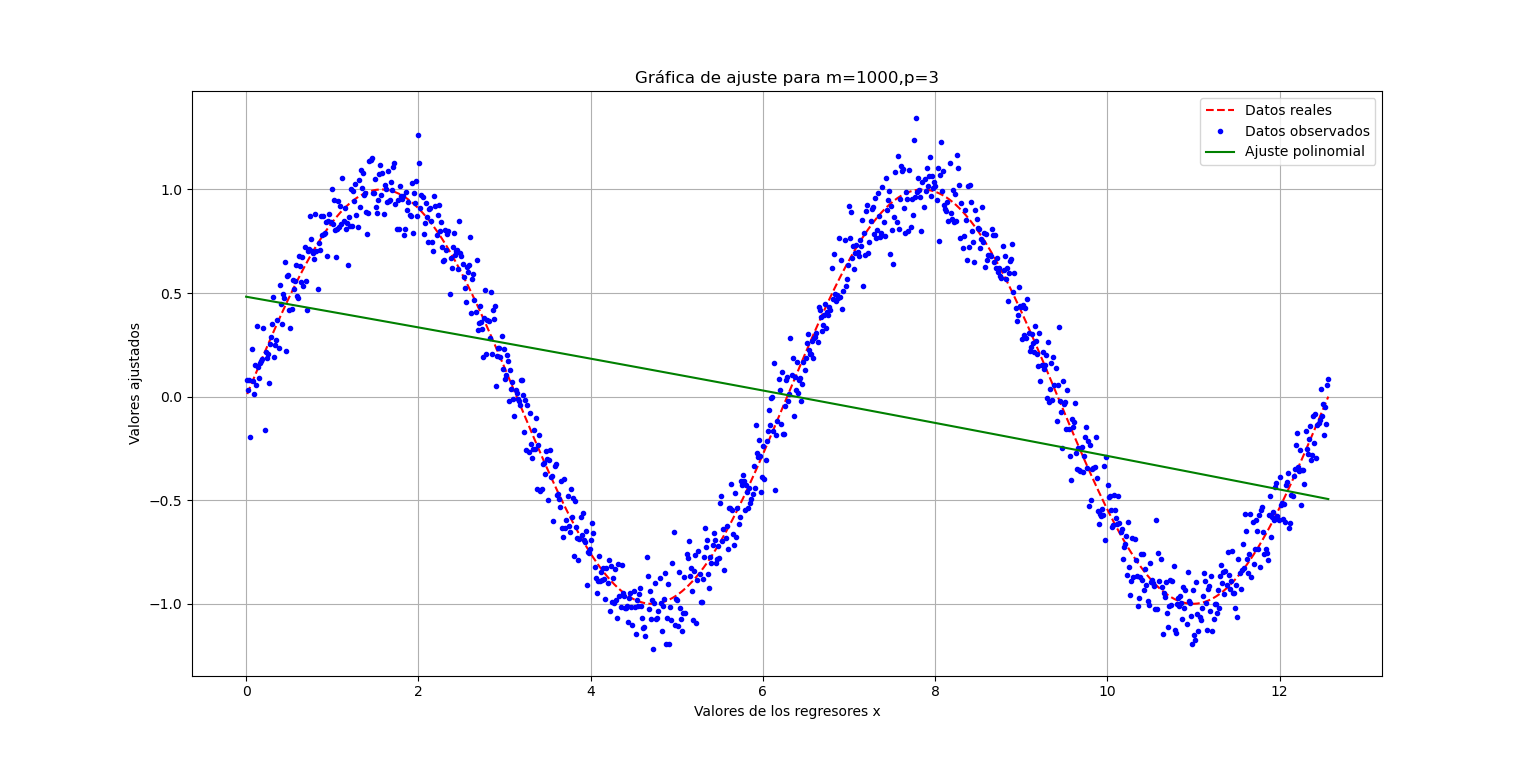
\includegraphics[width=0.7\linewidth]{5.png}
        \caption{}
    \end{figure}  
    \begin{figure}[h]
        \centering
        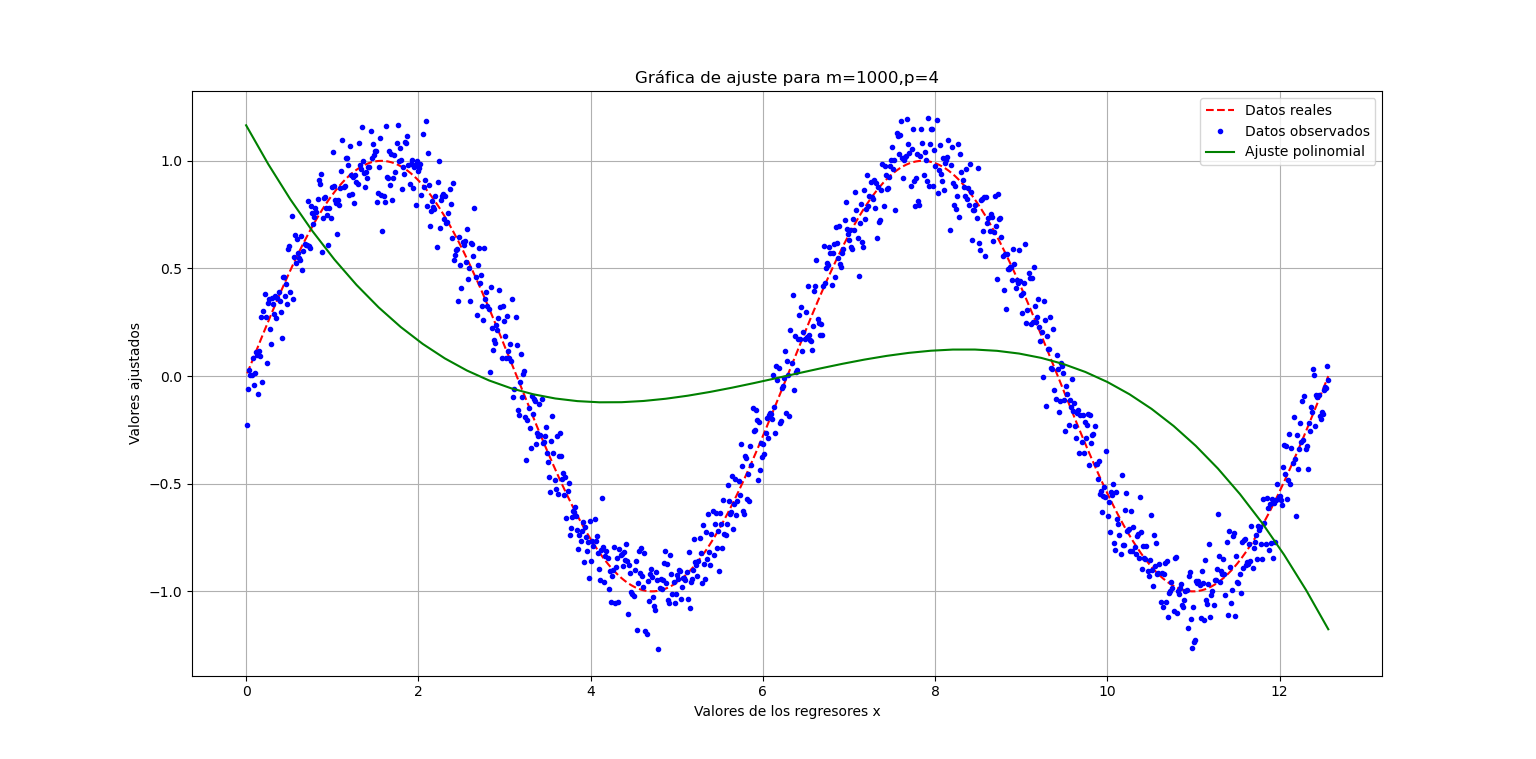
\includegraphics[width=0.7\linewidth]{6.png}
        \caption{}
    \end{figure}  
    \begin{figure}[h]
        \centering
        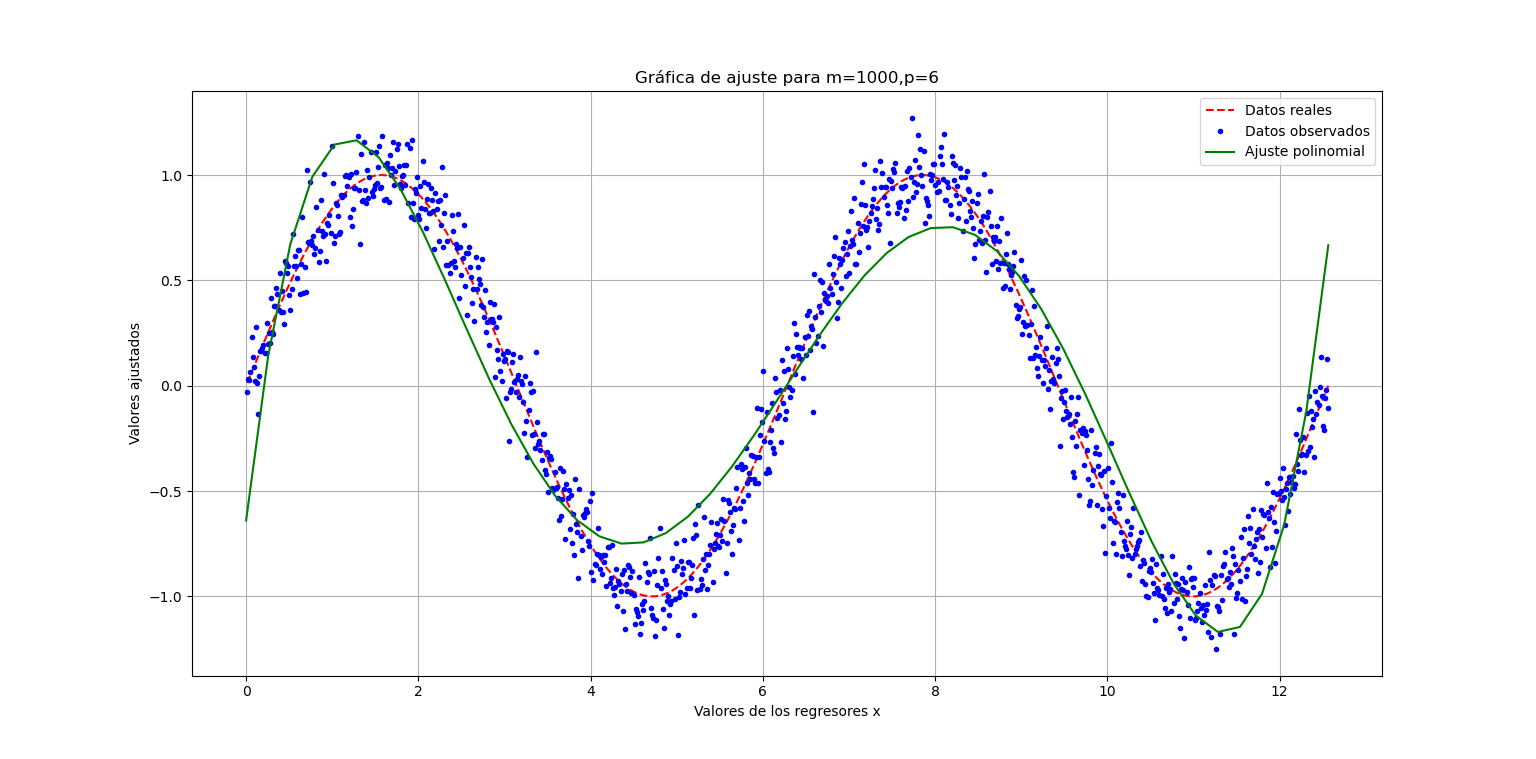
\includegraphics[width=0.7\linewidth]{7.png}
        \caption{}
    \end{figure}  
    \begin{figure}[h]
        \centering
        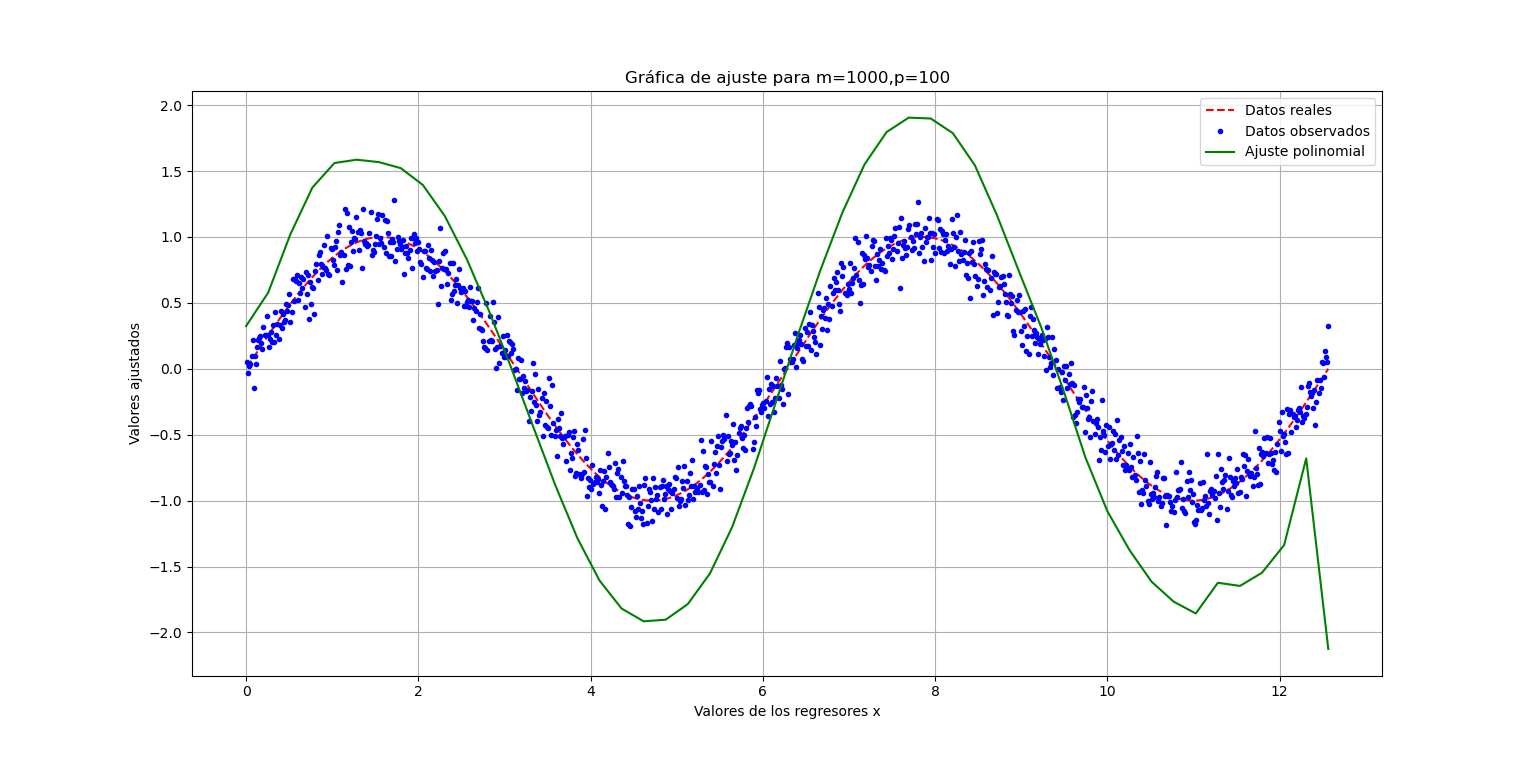
\includegraphics[width=0.7\linewidth]{8.png}
        \caption{}
    \end{figure}  
    \begin{figure}[h]
        \centering
        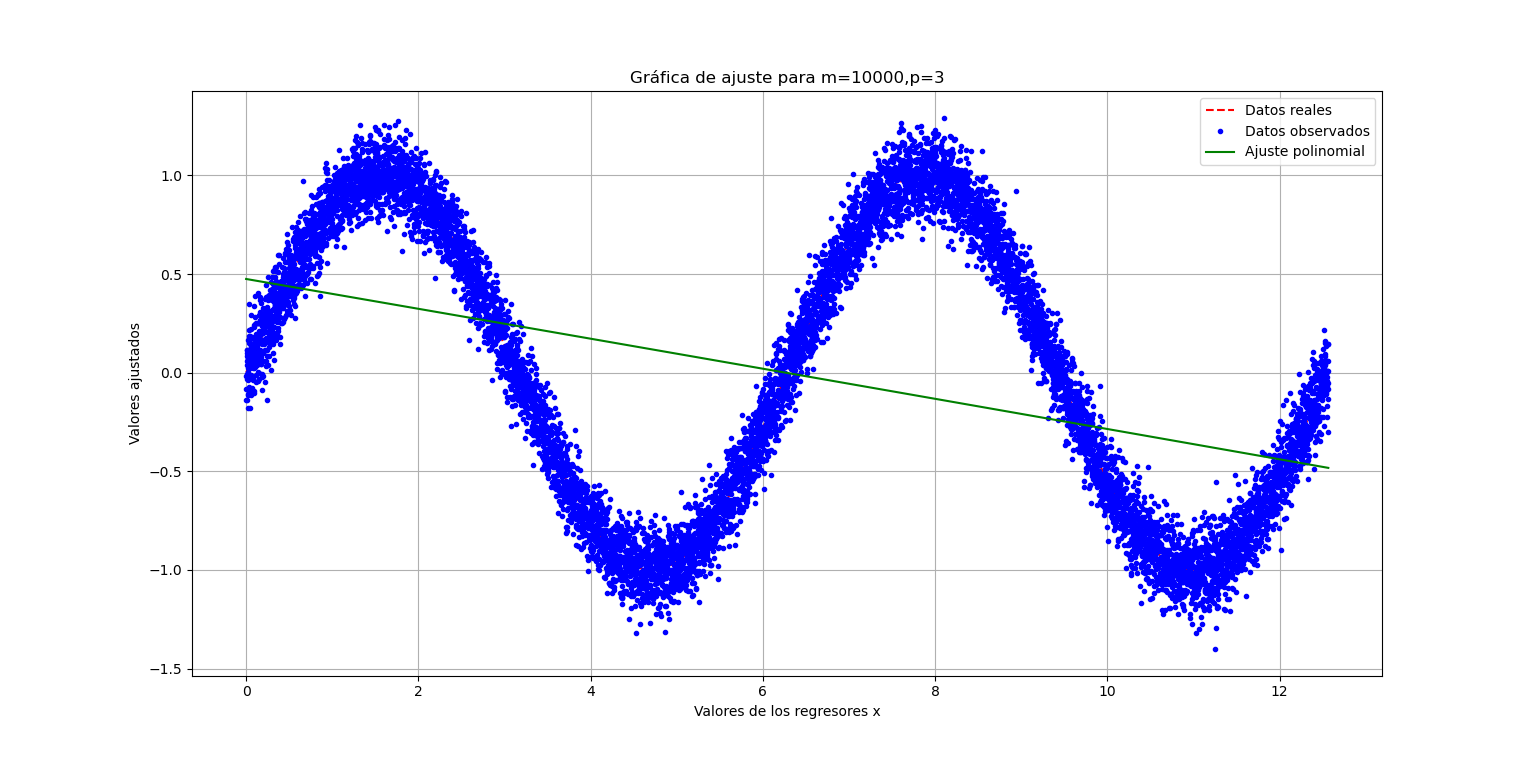
\includegraphics[width=0.7\linewidth]{9.png}
        \caption{}
    \end{figure}  
    \begin{figure}[h]
        \centering
        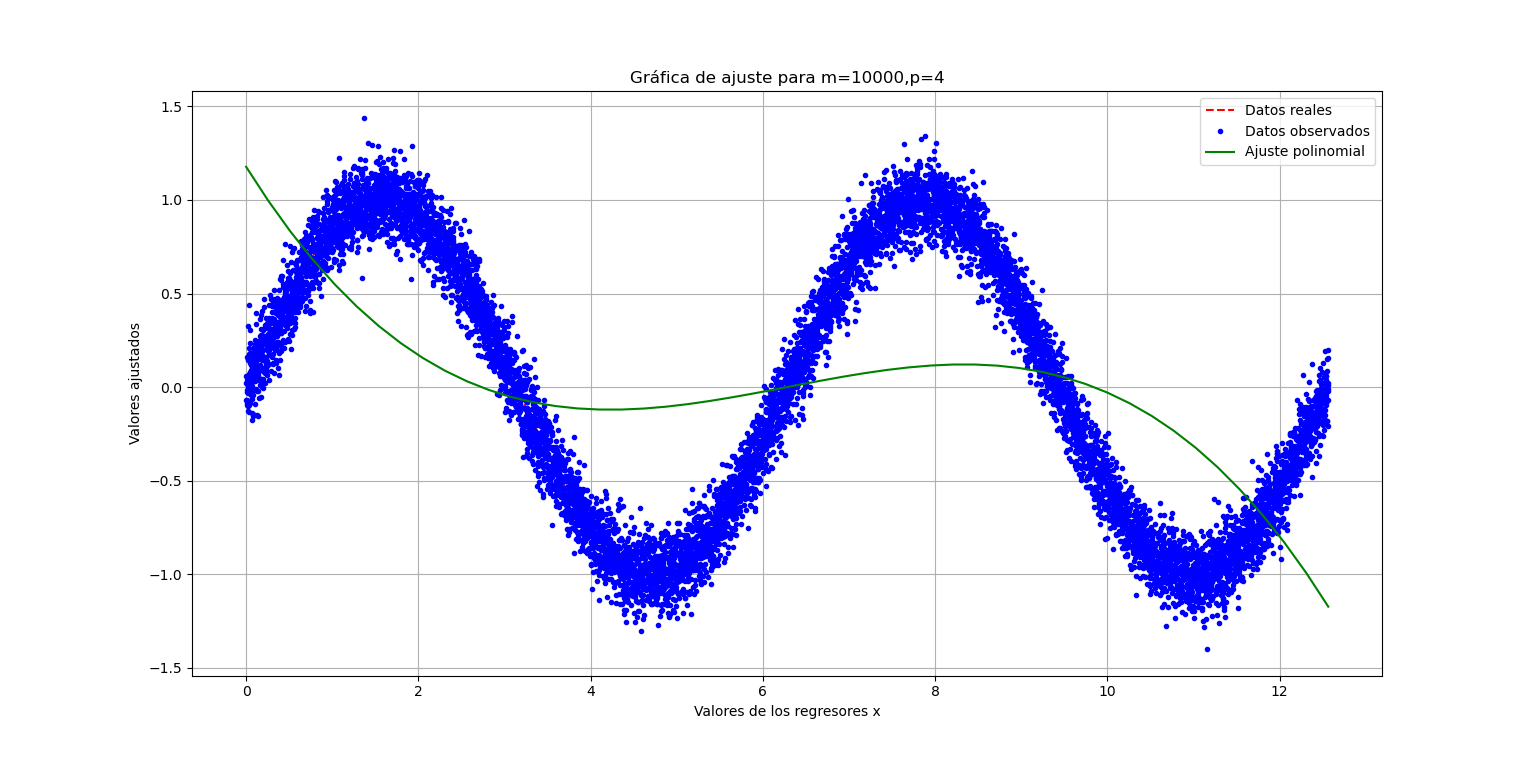
\includegraphics[width=0.7\linewidth]{10.png}
        \caption{}
    \end{figure}  
    \begin{figure}[h]
        \centering
        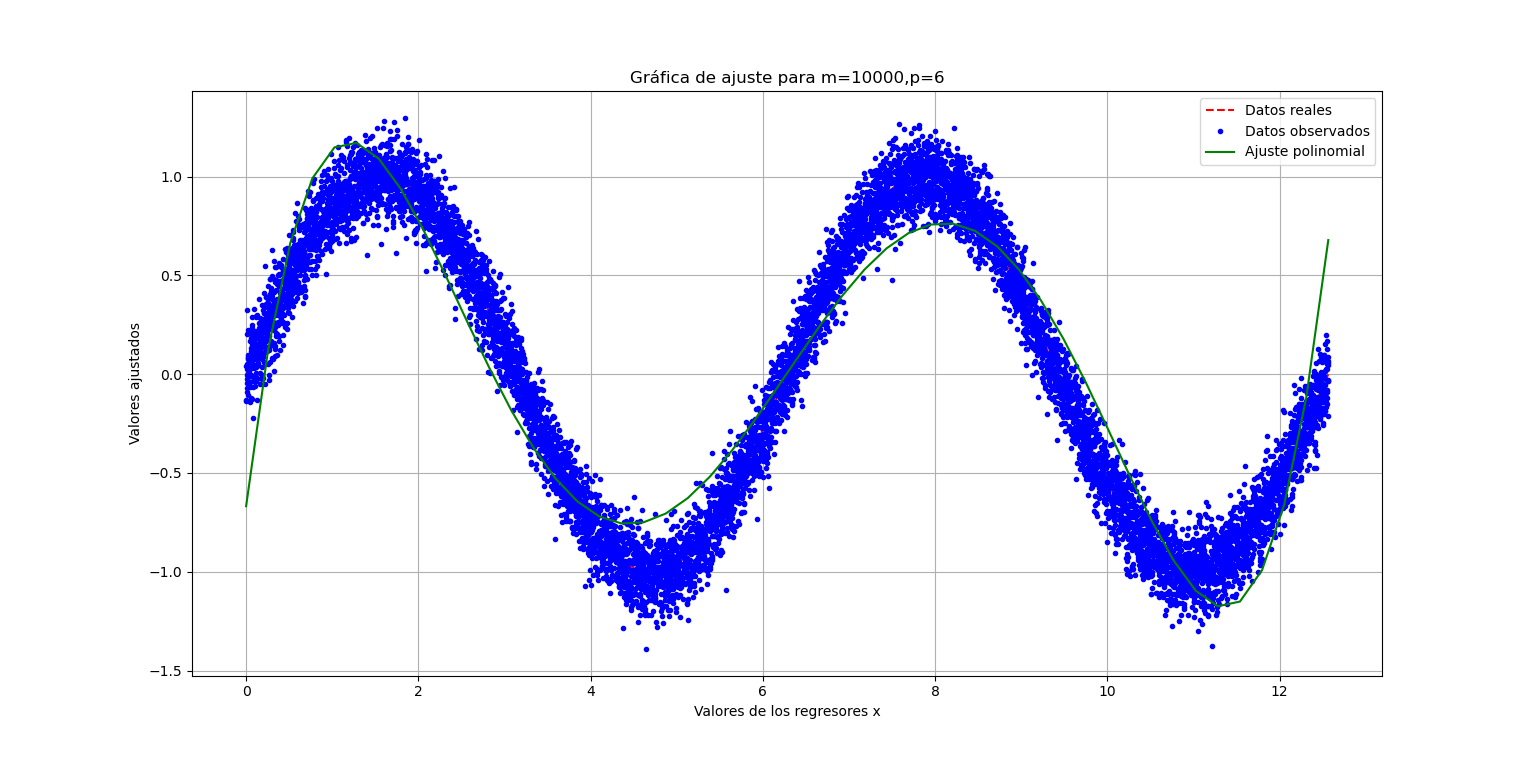
\includegraphics[width=0.7\linewidth]{11.png}
        \caption{}
    \end{figure}  
    \begin{figure}[h]
        \centering
        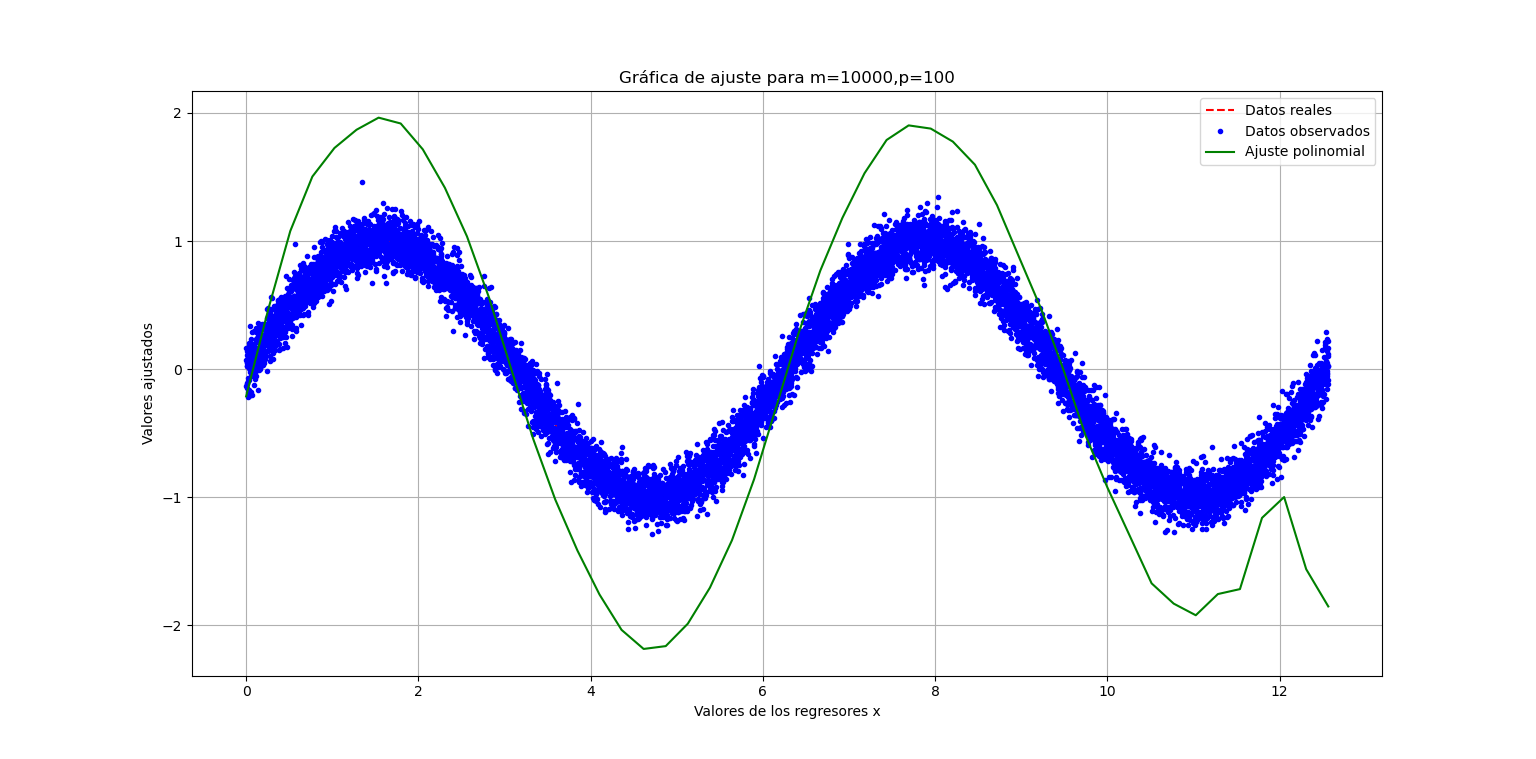
\includegraphics[width=0.7\linewidth]{12.png}
        \caption{}
    \end{figure}  
    Como podemos observar en las figuras 1 a 4 correspondientes al caso $m=100, p=3,4,6,100$,
    el ajuste polinomial es razonable en las primeras tres, mientras que en la última el
    ajuste es bastante malo. Este comportamiento no es para nada esperado, puesto que, por
    ejemplo, para el caso en el que $p=100$, se estaría ajustando un polinomio de grado
    99 a 100 puntos, lo que prácticamente debería otorgarnos una polinomio que conectara
    punto a punto los datos observados, fenómeno que no se observa.
     \newline

     El resto de ajustes presenta un problema similar. En particular, podemos observar
     que el ajuste polinomial se asemeja en cierto modo a una gráfica de $2\sen(x)$, en
     vez del $\sen(x)$ que se está tratando de ajustar. Este fenómeno se percibe fuertemente
     en las figuras 8 y 12 respectivamente. El ajuste en las demás figuras no es el que
     intuitivamente se esperaría, por ejemplo, en la figura 7, a intuición dice que puede
     mejorarse el polinomio que aproxime a los datos, sin embargo, el ajuste de ese polinomio
     es mejor que el que se presenta en la figura 8 por ejemplo.
     \newline

     Finalmente, realizamos la comparación con el algoritmo QR de scipy. Para ello, usamos
     la función 
     \begin{lstlisting}
     scipy.linalg.qr(- , mode='economic')   
     \end{lstlisting}
     el cual calcula QR reducido de acuerdo a la documentación de Scipy. El resultado es que
     la descomposición de Scipy es notoriamente mejor que la del QR implementado en este ejercicio,
     como se puede ver en la figura13.
     \begin{figure}[h]
        \centering
        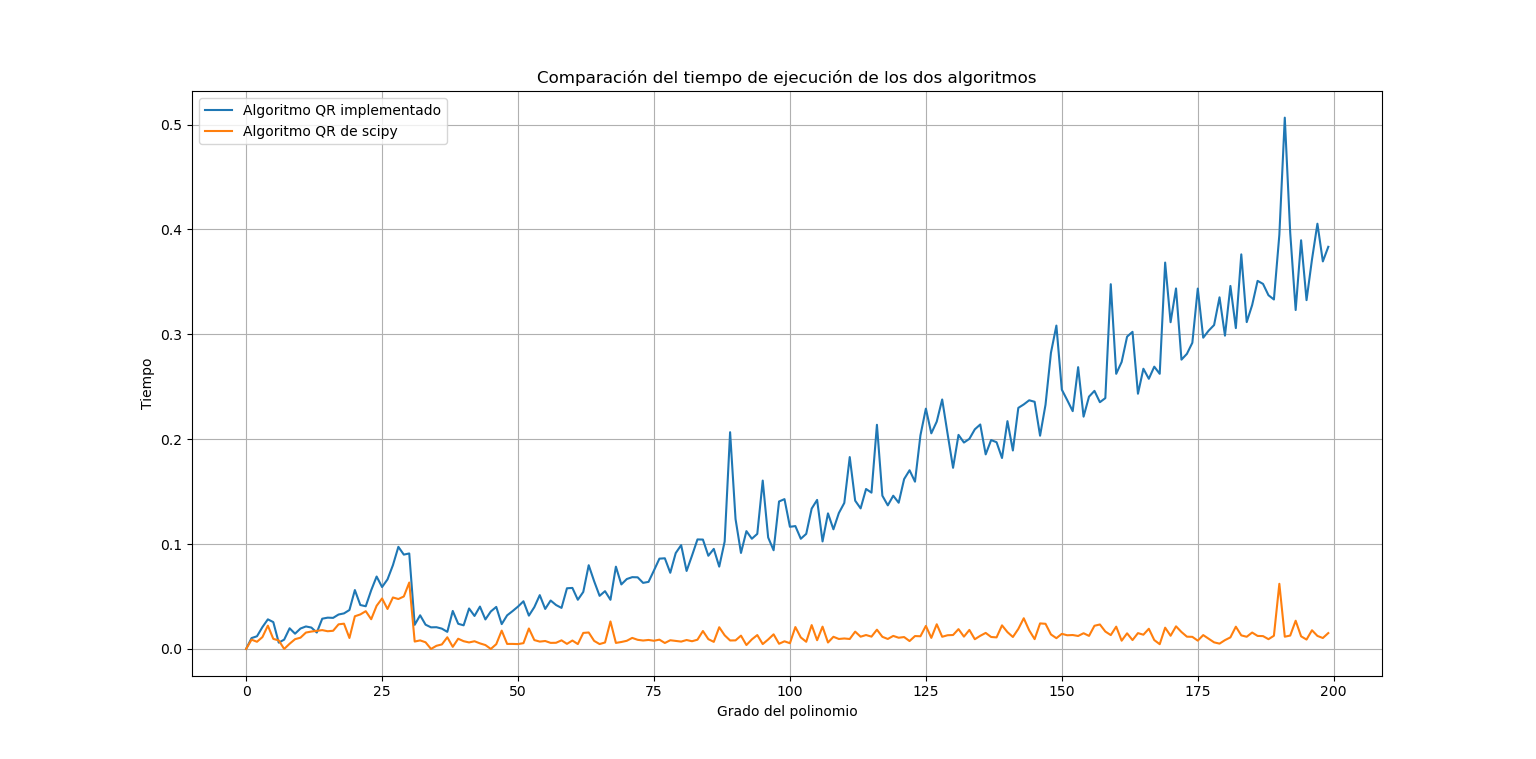
\includegraphics[width=\linewidth]{13.png}
        \caption{Tiempos de ejecución del algoritmo QR implementado vs QR de scipy.}
    \end{figure}

  

    \item Hacer $p=0.1n$, o sea, diez veces más observaciones que coeficientes en 
    la regresión. ¿Cuál es la $n$ máxima que puede manejar su computadora?\\

    \textbf{Solución:} Después de realizar varias pruebas, observamos dos comportamientos interesantes
    en ciertas cantidades:
    \begin{enumerate}
        \item \textbf{m=2800 vs m=2810:} aquí observamos que, cuando hay $m=2800$ datos con $p=280$ regresores (incluyendo el intercepto), 
        se tiene que el algoritmo trabaja 'correctamente' en el sentido de que el vector y la matriz resultante tienen valores 
        numéricos (aunque, como es posible observar en la figura, la mayoría de las respuestas del vector solución $s$ son cero.)
        \newline

        \begin{figure}[h]
            \centering
            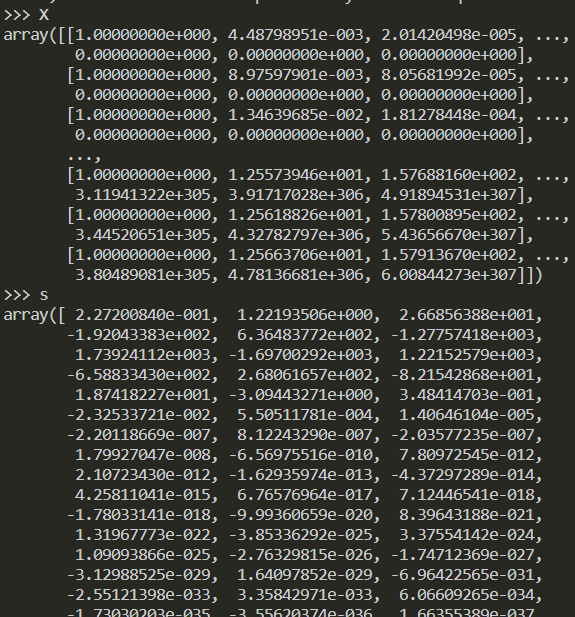
\includegraphics[width=0.5\linewidth]{m2800.png}
            \caption{Resultado del algoritmo cuando m=2800, p=280}
        \end{figure}

        \begin{figure}[h]
            \centering
            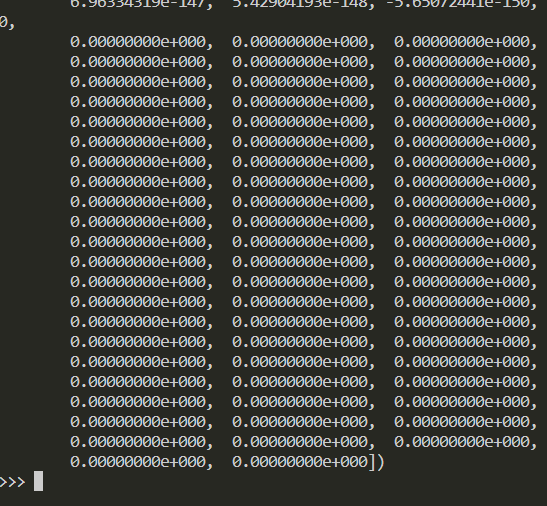
\includegraphics[width=0.5\linewidth]{m28002.png}
            \caption{Resultado del algoritmo cuando m=2800, p=280}
        \end{figure}

        No obstante, cuando el número de datos llega 2810, y el polinomio es de grado 281, se empiezan a obtener valores en la 
        matriz $X$ que interpretan como infinito, por lo que el vector empieza a regresar respuestas no numéricas 'nan', como 
        se puede observar en la figura. De esta forma, el algoritmo 'deja de ser útil' en $m=2810$.\\

        \begin{figure}[h]
            \centering
            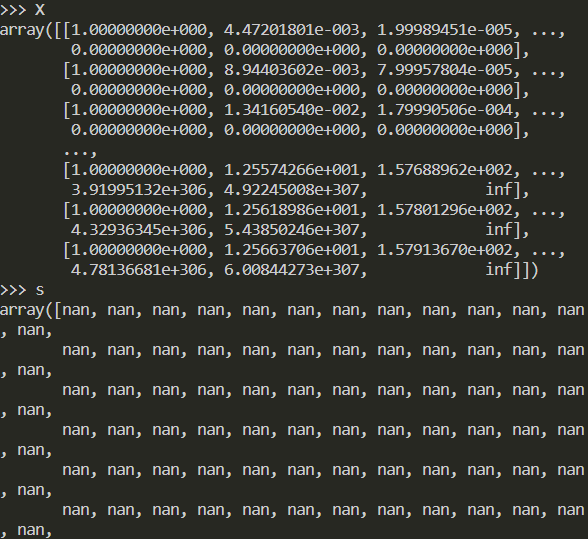
\includegraphics[width=0.5\linewidth]{m2810.png}
            \caption{Resultado del algoritmo cuando m=2810, p=281}
        \end{figure}

        \item \textbf{m=1540 vs m=1550:} a pesar de que técnicamente Python nos regresa una matriz $X$ y un vector
              de soluciones $s$ para el ítem $a)$, desde que $m=1550$, empiezan a surgir errores del tipo 'overflow', como se puede
              observar en las figuras, esto es, estamos ya fuera del rango que puede representarse con cierto
              número de dígitos en Python. Esto coincide precisamente con el primer instante en el que el vector solución 
              $s$ empieza a presentar ceros como parte de los coeficientes de la solución.

            \begin{figure}[h]
                \centering
                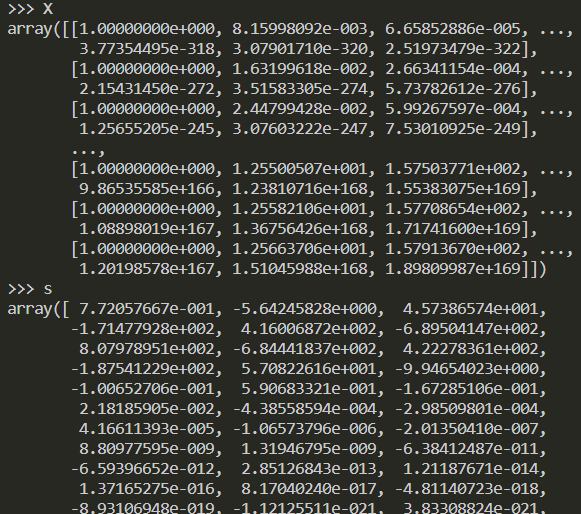
\includegraphics[width=0.5\linewidth]{m1540.png}
                \caption{Resultado del algoritmo cuando m=1540, p=154}
            \end{figure}      

            \begin{figure}[h]
                \centering
                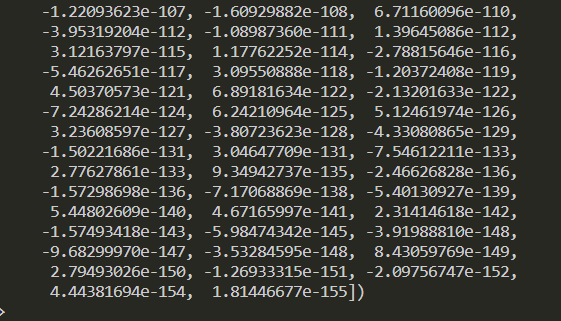
\includegraphics[width=0.5\linewidth]{m15402.png}
                \caption{Resultado del algoritmo cuando m=1540, p=154}
            \end{figure}       

            \begin{figure}[h]
                \centering
                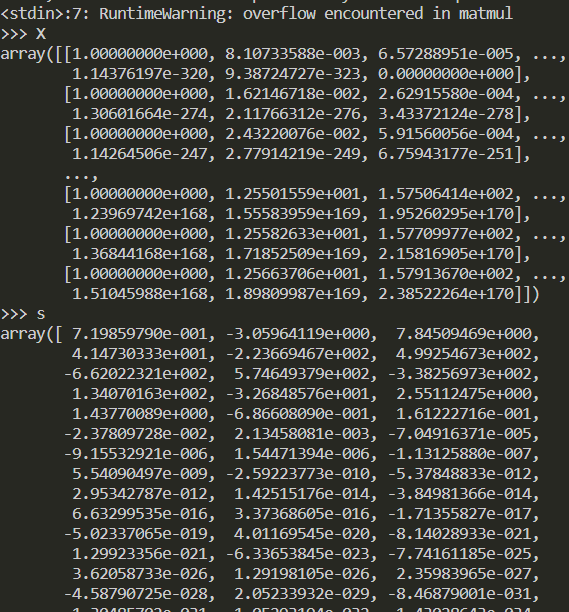
\includegraphics[width=0.5\linewidth]{m1550.png}
                \caption{Resultado del algoritmo cuando m=1550, p=155}
            \end{figure}

            \begin{figure}[h]
                \centering
                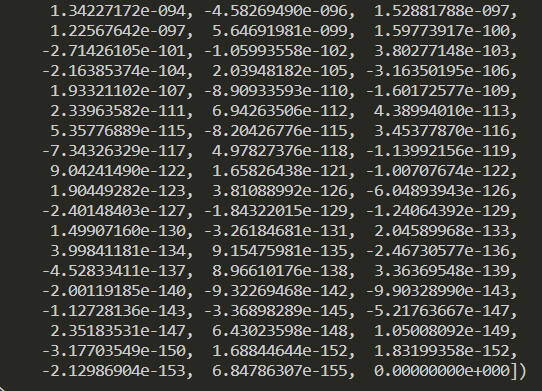
\includegraphics[width=0.5\linewidth]{m15502.png}
                \caption{Resultado del algoritmo cuando m=1550, p=155}
            \end{figure}

\end{enumerate}
\end{enumerate}
\end{document}